\documentclass[11pt,a4paper]{jsarticle}
\usepackage{amsmath,amssymb}
\usepackage{amsthm}
\usepackage{ascmac}
\usepackage{bm}
\usepackage[dvipdfmx]{graphicx}	% required for `\includegraphics' (yatex added)
\usepackage{setspace}           % required for `\doublespace'
\usepackage{tikz}
\usepackage{tikz-cd}
\usetikzlibrary{angles, positioning, shapes, arrows.meta, decorations.pathmorphing}
%\usetikzlibrary{intersections, calc, arrows, positioning, arrows.meta}
\usepackage{tcolorbox}  % 定理環境の装飾
\tcbuselibrary{skins, breakable, theorems}
\usepackage{xcolor}
\usepackage{natbib}
\usepackage{pxrubrica}
\usepackage[margin=30truemm, left=40truemm, right=40truemm]{geometry}
\usepackage{thmbox}     % required for theorem environment with side bar
%
\setlength{\parskip}{3mm} %段落間にスペースを入れる


% \pagestyle{myheadings}
% \markright{\footnotesize \sf 2022秋期「哲学者のための数学」授業資料(大塚淳) \ \ 配布禁止}


\theoremstyle{definition}
\newtheorem[S]{exercise}{練習問題}[section]
\newtheorem[S]{example}{事例}[section]
\newtheorem[S]{fact}{事実}[section]
\newtheorem[S]{attn}{注意}[section]
\newtheorem[S]{develop}{発展}[section]
\renewcommand{\theattn}{}

\newtcbtheorem[auto counter, number within=section]{rei}{事例}{
    breakable,
    coltitle=black,
    fonttitle=\bfseries,
    enhanced, colback=white, frame hidden, borderline west = {0.5pt}{5pt}{black},
%    number freestyle={\noexpand\thesection.\noexpand\arabic{\tcbcounter}}
}{rei}

\newtcbtheorem[auto counter, number within=section]{prop}{命題}{
    breakable,
    coltitle=black,
    fonttitle=\bfseries,
    enhanced, colback=white, frame hidden, borderline west = {0.5pt}{5pt}{black},
%    number freestyle={\noexpand\thesection.\noexpand\arabic{\tcbcounter}}
}{prop}

\newtcbtheorem[number within=section]{renshu}{練習問題}{
    breakable,
    coltitle=black,
    fonttitle=\bfseries,
    enhanced, colback=white, frame hidden, borderline west = {0.5pt}{5pt}{black}
}{renshu}


\newtcbtheorem[number within=section]{hatten}{発展}{
    breakable,
    coltitle=black,
    fonttitle=\bfseries,
    enhanced, colback=white, frame hidden, borderline west = {0.5pt}{5pt}{black}
}{renshu}


\newtcbtheorem[number within=section]{dfn}{定義}{
    fonttitle=\bfseries,
    enhanced, colback=white
}{dfn}


% Bold face capital letters:
\newcommand{\bfzero}{\boldsymbol{0}}
\newcommand{\bfone}{\boldsymbol{1}}
\newcommand{\bfA}{\boldsymbol{A}}
\newcommand{\bfB}{\boldsymbol{B}}
\newcommand{\bfC}{\boldsymbol{C}}
\newcommand{\bfD}{\boldsymbol{D}}
\newcommand{\bfE}{\boldsymbol{E}}
\newcommand{\bfF}{\boldsymbol{F}}
\newcommand{\bfG}{\boldsymbol{G}}
\newcommand{\bfH}{\boldsymbol{H}}
\newcommand{\bfI}{\boldsymbol{I}}
\newcommand{\bfJ}{\boldsymbol{J}}
\newcommand{\bfK}{\boldsymbol{K}}
\newcommand{\bfL}{\boldsymbol{L}}
\newcommand{\bfM}{\boldsymbol{M}}
\newcommand{\bfN}{\boldsymbol{N}}
\newcommand{\bfO}{\boldsymbol{O}}
\newcommand{\bfP}{\boldsymbol{P}}
\newcommand{\bfQ}{\boldsymbol{Q}}
\newcommand{\bfR}{\boldsymbol{R}}
\newcommand{\bfS}{\boldsymbol{S}}
\newcommand{\bfT}{\boldsymbol{T}}
\newcommand{\bfU}{\boldsymbol{U}}
\newcommand{\bfV}{\boldsymbol{V}}
\newcommand{\bfW}{\boldsymbol{W}}
\newcommand{\bfX}{\boldsymbol{X}}
\newcommand{\bfY}{\boldsymbol{Y}}
\newcommand{\bfZ}{\boldsymbol{Z}}

\newcommand{\bfa}{\boldsymbol{a}}
\newcommand{\bfb}{\boldsymbol{b}}
\newcommand{\bfc}{\boldsymbol{c}}
\newcommand{\bfd}{\boldsymbol{d}}
\newcommand{\bfe}{\boldsymbol{e}}
\newcommand{\bff}{\boldsymbol{f}}
\newcommand{\bfk}{\boldsymbol{k}}
\newcommand{\bfm}{\boldsymbol{m}}
\newcommand{\bfn}{\boldsymbol{n}}
\newcommand{\bfo}{\boldsymbol{o}}
\newcommand{\bfp}{\boldsymbol{p}}
\newcommand{\bfq}{\boldsymbol{q}}
\newcommand{\bfr}{\boldsymbol{r}}
\newcommand{\bfs}{\boldsymbol{s}}
\newcommand{\bft}{\boldsymbol{t}}
\newcommand{\bfu}{\boldsymbol{u}}
\newcommand{\bfv}{\boldsymbol{v}}
\newcommand{\bfw}{\boldsymbol{w}}
\newcommand{\bfx}{\boldsymbol{x}}
\newcommand{\bfy}{\boldsymbol{y}}
\newcommand{\bfz}{\boldsymbol{z}}



% BB (???) capital letters:
\newcommand{\bbA}{\mathbb{A}}
\newcommand{\bbB}{\mathbb{B}}
\newcommand{\bbC}{\mathbb{C}}
\newcommand{\bbD}{\mathbb{D}}
\newcommand{\bbE}{\mathbb{E}}
\newcommand{\bbF}{\mathbb{F}}
\newcommand{\bbG}{\mathbb{G}}
\newcommand{\bbI}{\mathbb{I}}
\newcommand{\bbN}{\mathbb{N}}
\newcommand{\bbP}{\mathbb{P}}
\newcommand{\bbQ}{\mathbb{Q}}
\newcommand{\bbR}{\mathbb{R}}
\newcommand{\bbU}{\mathbb{U}}
\newcommand{\bbV}{\mathbb{V}}
\newcommand{\bbX}{\mathbb{X}}
\newcommand{\bbY}{\mathbb{Y}}
\newcommand{\bbZ}{\mathbb{Z}}
\newcommand{\bbone}{{\ifmmode\mathrm{1\!l}\else\mbox{\(\mathrm{1\!l}\)}\fi}}


% Caligraphic math capital letters:
\newcommand{\mcalA}{\mathcal{A}}
\newcommand{\mcalB}{\mathcal{B}}
\newcommand{\mcalC}{\mathcal{C}}
\newcommand{\mcalD}{\mathcal{D}}
\newcommand{\mcalE}{\mathcal{E}}
\newcommand{\mcalF}{\mathcal{F}}
\newcommand{\mcalG}{\mathcal{G}}
\newcommand{\mcalH}{\mathcal{H}}
\newcommand{\mcalI}{\mathcal{I}}
\newcommand{\mcalJ}{\mathcal{J}}
\newcommand{\mcalK}{\mathcal{K}}
\newcommand{\mcalL}{\mathcal{L}}
\newcommand{\mcalM}{\mathcal{M}}
\newcommand{\mcalN}{\mathcal{N}}
\newcommand{\mcalO}{\mathcal{O}}
\newcommand{\mcalP}{\mathcal{P}}
\newcommand{\mcalQ}{\mathcal{Q}}
\newcommand{\mcalS}{\mathcal{S}}
\newcommand{\mcalT}{\mathcal{T}}
\newcommand{\mcalU}{\mathcal{U}}
\newcommand{\mcalV}{\mathcal{V}}
\newcommand{\mcalX}{\mathcal{X}}
\newcommand{\mcalY}{\mathcal{Y}}
\newcommand{\mcalZ}{\mathcal{Z}}

% Graph nodes notations:
\newcommand{\PA}{\mathit{PA}}
\newcommand{\bfPA}{\mathbf{PA}}
\newcommand{\CH}{\mathit{CH}}
\newcommand{\bfCH}{\mathbf{CH}}
\newcommand{\DS}{\mathit{DS}}
\newcommand{\bfDS}{\mathbf{DS}}
\newcommand{\ND}{\mathit{ND}}
\newcommand{\bfND}{\mathbf{ND}}
\newcommand{\AN}{\mathit{an}}
\newcommand{\bfAN}{\mathbf{an}}
\newcommand{\pa}{\mathit{pa}}
\newcommand{\bfpa}{\mathbf{pa}}
\newcommand{\ch}{\mathit{ch}}
\newcommand{\bfch}{\mathbf{ch}}
\newcommand{\ds}{\mathit{ds}}
\newcommand{\bfds}{\mathbf{ds}}
\newcommand{\nd}{\mathit{nd}}
\newcommand{\bfnd}{\mathbf{nd}}
\newcommand{\an}{\mathit{an}}
\newcommand{\bfan}{\mathbf{an}}



\DeclareMathOperator*{\argmax}{arg\,max}
\DeclareMathOperator*{\argmin}{arg\,min}
\DeclareMathOperator*{\argsup}{arg\,sup}
\DeclareMathOperator*{\arginf}{arg\,inf}
\DeclareMathOperator{\erfc}{erfc}
\DeclareMathOperator{\diag}{diag}
\DeclareMathOperator{\cum}{cum}
\DeclareMathOperator{\sgn}{sgn}
\DeclareMathOperator{\tr}{tr}
\DeclareMathOperator{\spn}{span}
\DeclareMathOperator{\adj}{adj}
\DeclareMathOperator{\E}{\mathbb{E}}
\DeclareMathOperator{\var}{Var}
\DeclareMathOperator{\cov}{Cov}
\DeclareMathOperator{\corr}{corr}
\DeclareMathOperator{\sech}{sech}
\DeclareMathOperator{\sinc}{sinc}
\DeclareMathOperator*{\lms}{l.i.m.\,}
\newcommand{\varop}[1]{\var\left[{#1}\right]}
\newcommand{\covop}[2]{\cov\left({#1},{#2}\right)}
\newcommand{\T}{^\textrm{T}}
\newcommand\indep{\protect\mathpalette{\protect\independenT}{\perp}}
\def\independenT#1#2{\mathrel{\rlap{$#1#2$}\mkern2mu{#1#2}}}

\newcommand{\bfalpha}{\boldsymbol{\alpha}}
\newcommand{\bfbeta} {\boldsymbol{\beta}}
\newcommand{\bfgamma}{\boldsymbol{\gamma}}
\newcommand{\bfeta}  {\boldsymbol{\eta}}
\newcommand{\bftheta}{\boldsymbol{\theta}}
\newcommand{\bflambda}   {\boldsymbol{\lambda}}
\newcommand{\bfmu}   {\boldsymbol{\mu}}
\newcommand{\bfnu}   {\boldsymbol{\nu}}
\newcommand{\bfxi}   {\boldsymbol{\xi}}
\newcommand{\bfpsi}  {\boldsymbol{\psi}}
\newcommand{\bfphi}   {\boldsymbol{\phi}}
\newcommand{\bfrho}   {\boldsymbol{\rho}}
\newcommand{\bfvarepsilon}{\boldsymbol{\varepsilon}}
%\newcommand{\qed}{{qed}}
%\newcommand{\eqalignno}[1]{\begin{array}{ccccccc}#1\end{array}}

\newcommand{\bfGamma}{\boldsymbol{\Gamma}}
\newcommand{\bfTheta}{\boldsymbol{\Theta}}
\newcommand{\bfLambda}   {\boldsymbol{\Lambda}}
\newcommand{\bfPsi}  {\boldsymbol{\Psi}}
\newcommand{\bfPhi}   {\boldsymbol{\Phi}}
\newcommand{\bfSigma}  {\boldsymbol{\Sigma}}
\newcommand{\bfOmega}  {\boldsymbol{\Omega}}


% DISTRIBUTIOoNS: 
\newcommand{\normal}{\mathcal{N}}
\newcommand{\binomial}{\mathcal{B}}
\newcommand{\multinomial}{\mathcal{M}}
\newcommand{\exponential}{\mathcal{E}}
\newcommand{\geometric}{\mathcal{G}}
\newcommand{\poisson}{\mbox{Poisson}}
\newcommand{\uniform}{\mbox{Uniform}}

% Logic
\newcommand{\true}{\texttt{true}}
\newcommand{\false}{\texttt{false}}


%PSTricks (commande for latent nodes)
\newcommand{\lnode}[4]{ \cnode(#1){#2}{#3}\rput(#1){\footnotesize#4} }

% KEEPING TRACK OF WORK
\newcommand{\todo}[1]
{
{\color{red}{
[TODO: #1]}}
\addcontentsline{toc}{subsection}{TO DO: #1}
}

\newcommand{\fixme}[1]{{\color{red}{#1}}}

\newenvironment{answer}[1]
{\par \color{blue}{#1}}
{}


\newcommand{\note}[2]
{
{\color{red}{
[#1: #2]}}
}




\makeatletter
% define \citepos for posesive citation (e.g. Otsuka's (2015))
\DeclareRobustCommand\citepos
  {\begingroup
   \let\NAT@nmfmt\NAT@posfmt% ...except with a different name format
   \NAT@swafalse\let\NAT@ctype\z@\NAT@partrue
   \@ifstar{\NAT@fulltrue\NAT@citetp}{\NAT@fullfalse\NAT@citetp}}

\let\NAT@orig@nmfmt\NAT@nmfmt
\def\NAT@posfmt#1{\NAT@orig@nmfmt{#1's}}
\makeatother




% Code for drawing color circle used in topology (pathconnectedness)
\usepackage{xparse}
\ExplSyntaxOn

\keys_define:nn { colour_transition_circle } {
    inner   .fp_set:N   = \l__inner_radius,
    inner   .initial:n  = {2},
    outer   .fp_set:N   = \l__outer_radius,
    outer   .initial:n  = {3},
    angle   .fp_set:N   = \l__start_angle,
    angle   .initial:n  = {0}
}

\NewDocumentCommand \ColourTransitionCircle { O{} m } {
\group_begin:
    \keys_set:nn { colour_transition_circle } {#1}
    \clist_clear:N \l_tmpa_clist
    \clist_map_inline:nn {#2} {
        \clist_put_right:Nn \l_tmpa_clist {##1}
        %\clist_put_right:Nn \l_tmpa_clist {##1}
    }
    \exp_args:Nx \col_trans_circ:n \l_tmpa_clist
\group_end:
}

\cs_new_protected:Npn \col_trans_circ:n #1 {
    \int_step_inline:nnnn {1} {1} {\clist_count:n {#1} - 1} {
        \path[top~color=\clist_item:nn {#1} {##1}, bottom~color=\clist_item:nn {#1} {##1+1}, shading~angle={270-(180-360/\clist_count:n {#1})/2+(##1-1)*360/\clist_count:n {#1}+\fp_use:N \l__start_angle}] ({\fp_use:N \l__inner_radius*cos((##1-1)*360/\clist_count:n {#1}+\fp_use:N \l__start_angle)},{\fp_use:N \l__inner_radius*sin((##1-1)*360/\clist_count:n {#1}+\fp_use:N \l__start_angle)}) arc[radius = \fp_use:N \l__inner_radius, start~angle={(##1-1)*360/\clist_count:n {#1}+\fp_use:N \l__start_angle}, delta~angle=360/\clist_count:n {#1}] -- ({\fp_use:N \l__outer_radius*cos(##1*360/\clist_count:n {#1}+\fp_use:N \l__start_angle)},{\fp_use:N \l__outer_radius*sin(##1*360/\clist_count:n {#1}+\fp_use:N \l__start_angle)}) arc[radius = \fp_use:N \l__outer_radius, start~angle={##1*360/\clist_count:n {#1}+\fp_use:N \l__start_angle}, delta~angle=-360/\clist_count:n {#1}] -- cycle;
    }
    \path[top~color=\clist_item:nn {#1} {\clist_count:n {#1}}, bottom~color=\clist_item:nn {#1} {1}, shading~angle={180-180/\clist_count:n {#1}+\fp_use:N \l__start_angle}]({\fp_use:N \l__inner_radius*cos((\clist_count:n {#1}-1)*360/\clist_count:n {#1}+\fp_use:N \l__start_angle)},{\fp_use:N \l__inner_radius*sin((\clist_count:n {#1}-1)*360/\clist_count:n {#1}+\fp_use:N \l__start_angle)}) arc[radius = \fp_use:N \l__inner_radius, start~angle={(\clist_count:n {#1}-1)*360/\clist_count:n {#1}+\fp_use:N \l__start_angle}, delta~angle=360/\clist_count:n {#1}] -- ({\fp_use:N \l__outer_radius*cos(\clist_count:n {#1}*360/\clist_count:n {#1}+\fp_use:N \l__start_angle)},{\fp_use:N \l__outer_radius*sin(\clist_count:n {#1}*360/\clist_count:n {#1}+\fp_use:N \l__start_angle)}) arc[radius = \fp_use:N \l__outer_radius, start~angle={\clist_count:n {#1}*360/\clist_count:n {#1}+\fp_use:N \l__start_angle}, delta~angle=-360/\clist_count:n {#1}] -- cycle;
}

\ExplSyntaxOff


\usepackage{tikz}
\usetikzlibrary{intersections, calc, arrows, positioning, arrows.meta}

\begin{document}


\title{5. モノイド・群}
\author{2022秋期「哲学者のための数学」授業資料(大塚淳)}
\date{ver. \today}
\maketitle

\section{モノイドとは何か,なぜそれを学ぶのか}
前章で見た位相は,空間に関する幾何学的な概念であった.
一方本章の主題となるモノイドや群は,本質的に代数的な「計算」にまつわる概念である.
よって我々は,代数,幾何と来て我々は再び代数の世界に戻ってきた.

文系の学生にとって,「位相」という言葉は耳にしたことくらいはあっても,「モノイド」や「群」となると聞いたこともない,という人も多いかもしれない.
しかし実のところ我々は皆,小学生のころからモノイドや群に親しんでいる.
というのも,足し算や掛け算などはまさにこのモノイドや群の作用に他ならないからだ.
モノイドや群は,そうした四則演算を始めとした「演算」一般の最もプリミティブな形を抜き出したものと言える.
それ以外にも,モノイドは対象や系の変化・発展を表すために用いられるし,また群はモノの対称性(symmetry)の数学的な表現を与える.
そしてこの対称性という考え方は,物理学における「法則性」という考えを裏から支えるものであり,また哲学的には客観性の概念と深い結び付きを持っている.
こうしたことから,モノイドや群は非常に広範な科学的・哲学的含意を有している.

現代物理学を始め様々な科学で応用される群論は,極めて高度に発展しており,その全体像を掴むことを容易ではない.
しかしその基本的な考え方はこれ以上ないくらいシンプルである.
ここではその本質的な点のみに的を絞って紹介したい.
そこから得られるモノイドや群は,数学者や物理学者からしたらおもちゃみたいに簡単なものでしかないかもしれないが,その哲学的含意を考えるには十分であろう.

\section{モノイド}
まずは例に倣い,集合をベースにモノイドを定義しよう.

\begin{dfn}[モノイド]
集合$M$上に,積と呼ばれる二項写像$\circ: M \times M \to M$が定義されており,以下の条件を満たすとき,組$(M, \circ, i)$を\emph{モノイド}(monoid)という.
\begin{enumerate}
 \item $M$の任意の元$l, m, n$に対して,結合律$(l \circ m) \circ n = l \circ (m \circ n)$がなりたつ.
 \item \emph{単位元}(identity element)と呼ばれる元$i \in M$が存在して,$M$の任意の元$m$に対して,$i \circ m = m \circ i = m$がなりたつ.
\end{enumerate} 
\end{dfn}

これだけである.
つまりモノイドとは,その2つの元$m,n$をある元$m \circ n$に対応させるモノイド演算$\circ$が備わっているような集合である.
公理1は,この演算が結合律を満たすこと,そして公理2はこの演算において「何もしない」単位元が存在することを言っている.
しばしば演算記号は省略され,$m \circ n$は$mn$のように書かれる.
また誤解が生じないときは,演算や単位元を明示せずに単に$M$がモノイドである,というように言うこともある.


\begin{example}
ゼロを含む自然数$\bbN$(つまり非負整数)は,二項演算$+$とモノイドをなす.ここでの単位元は$0$である.
実際任意の自然数$x, y, z$について,$(x+y)+z = x + (y+z)$かつ$0 + x = x + 0 = x$. 
同様に,$\bbN$が乗算$\times$についてもモノイドとなることを確認せよ(その単位元はなんだろうか).
%また明らかなように,上の議論は自然数の代わりに有理数$\bbQ$,実数$\bbR$のゼロ以上の部分を用いても成立する.
\end{example}

\begin{example}
足し算についての上の議論は,自然数の代わりに有理数$\bbQ$,実数$\bbR$のゼロ以上の部分を用いても成立する.
例えば$\bbR^+ := \{ x \in \bbR | x \geq 0 \}$と定義すると,$(\bbR^+, +, 0)$はモノイドである.
(負の部分はどうなるのか,と思うかもしれないが,これはあとで群を定義するときに見る.)
\end{example}

モノイドの演算が具体的にどうなっているのかは,それぞれの元のペアの演算結果を明示することによって表示できる.
例えば,お馴染みの「九九の表」は,自然数の掛け算モノイドの演算を表で表したものだ:
\[
\begin{array}{c|cccccc}
       & 1 & 2 & 3 & \dots & m & \dots \\ \hline
     1 & 1 & 2 & 3 & \dots & n & \dots \\ 
     2 & 2 & 4 & 6 & \dots & 2n & \dots \\ 
     3 & 3 & 6 & 9 & \dots & 9n & \dots \\ 
     \vdots & \vdots & \vdots & \vdots & & \vdots & \\
     m & m & m2 & m3 & \cdots & mn & \cdots \\
     \vdots & \vdots & \vdots & \vdots & & \vdots & \\
\end{array}
\]
九九表の各マスは,モノイド$(\bbN, \times, 1)$の1から9までの各元(一番左の列)が,それぞれ1から9までの元(一番上の行)をどの自然数に対応させるかを表している.
すべてのモノイド演算は,原理的にこうした表(「積表」という)によって表すことができる.
つまり我々は小学生のころからモノイドを知っていたのである!


\begin{develop}
我々は今まで,(非負)実数$\bbR$を様々な数学的構造として見てきた.
集合として見ると(2章),それは$\aleph_1$の濃度を持つ不可算無限集合なのだった.
3章ではその要素の間に大小関係$\leq, \geq$を入れた全順序集合として見た.
4章では,実数が開区間$(a,b)$からなる開集合を持つ位相空間であることを確認した.
そしてここでは,二項演算$+$および$\times$が定義されたモノイドとして定義した.
このように,同じ「実数の集合」でも様々な顔を持ち,それらの顔はすでに見たような公理によって構成される.
我々が普段何気なく使う実数は,実はこうした顔全てをあわせもつ存在なのである.

 もちろん,実数の特徴づけはこれで終わりなわけではない.
 まず引き算と割り算の導入がまだであるし(これは以下で群のところで見る),またここで導入した足し算と掛け算が互いにどう関係し合うのか(例えば分配法則$a(b+c) = ab + ac$が満たされるか)などは,別個の公理によって定めなければならない.
 このためにはさらに\emph{環}(ring),\emph{体}(field)といった概念を導入しなければならいのだが,本授業ではそこまでは扱わない.
\end{develop}


\section{モノイド作用}
モノイドは,ある対象について作用を加えたときにどう変化するか,あるいは状態がどう変遷していくか,というダイナミックな過程をモデル化するためによく用いられる.
その鍵になるのが,次に見る\emph{モノイド作用}(monoid action)の概念である.

準備として,まず上で見たモノイド演算を別の仕方で捉えてみたい.
例えば足し算のモノイドでは,演算$+$は2つの整数(e.g., $5, 7$)をとって1つの整数($12$)を返す2項関数なのだった.
しかし同様の事態を,全てのモノイド元$m$は,他のモノイド元$n$に「$m$を足す」1項関数,すなわち$m:M \to M, n \mapsto m+n$である,と表すこともできるだろう.
これはつまり,例えば具体的な数7を,「7を足す」作用として考えよう,ということだ.
モノイド元の合成は作用の合成,例えば$m+n$は「$m$を足してから$n$を足す」という一つの作用となり,また単位元$0$は「$0$を足す」(つまり何も変えない)という作用である.
このようにモノイドは,「自分自身に働きそれを変える作用」として考えることができる.

同様にして,モノイド$M$を自身以外の集合$X$に対して作用させてみようというのが,モノイド作用の基本的な考え方である.
つまり各モノイド元を$X$から$X$への1項関数とみる,あるいは同じことだが$M \times X \to X$の2項関数としてモノイド演算を考えよう,ということだ:

\begin{dfn}
 $(M, \circ, i)$をモノイド,$X$を集合とする.
 モノイド$M$の集合$X$への(左)\emph{$M$-作用(M-act)}とは,写像
 \[
  M \times X \to X, \ \ \ \ (m, x) \mapsto mx
 \]
 であり,以下を満たすものである:
 \begin{enumerate}
  \item 任意の$x \in X$について,$ix = x$.
  \item 任意の$m, n \in M$と任意の$x \in X$に対して,$m(nx) = (mn)x$.
 \end{enumerate}
\end{dfn}
%$M$を$X$への作用とみなすということは,それぞれのモノイド元$m \in M$を,$X \to X$の写像としてみなすということである.
上の要件1は単位元$i$が「何もしない」恒等写像$i(x)=x$であること,
要件2はモノイド元の結合が写像の合成になっている(つまり$x$を$n$で飛ばしてから$m$で飛ばすのと,モノイド合成$mn$したもので飛ばすものが等しい)ということを述べている.
この定義の集合$X$を$M$にすると,モノイドの定義2.1が復元されることを確認しよう.
つまりすべてのモノイドは自分自身へのモノイド作用だといえる.\footnote{左作用についての注.}

モノイド作用をイメージするためには,$X$を何らかの対象が持つ状態の集合とし,モノイドの各元は各状態に対して働いてそれを変化させるもの,というように考えると良い.例えば次の例を考えてみよう.
\begin{example}
 3つの状態$X := \{H(appy), C(alm), S(ad)\}$をとり得るロボットを考える.
 このロボットに対する可能な入力として$M := \{\text{ほめる}, \text{しかる}, \text{放置}\}$の3つの選択肢があるとする.
 ロボットの状態は,その時の状態と入力に応じて以下のように変化するとする:
 \[
\begin{array}{c|ccc}
       & S & C & H \\ \hline
     \text{ほめる} & C & H & H \\
     \text{しかる} & S & S & S \\ 
     \text{放置}   & S & C & H\\
\end{array}
\]
この表の各マスは,ロボットが上端の行で示される各状態にあるとき,左端列の入力を与えるとどう変化するかを表している(例えば左上は,状態$S$(Sad)のときに「ほめる」と状態が$C$(Calm)になることを表す).
これは以前見た積表と同様にモノイド演算を表しており,入力$M$はロボットの状態$X$へのモノイド作用を与える(単位元は「放置」).

 
ちなみに同様の演算は,図\ref{robot}のような\emph{状態遷移図}(state transition diagram)によっても表すことができる.
状態集合を持ち,その間の状態遷移関係が定まっているような機械を,\emph{オートマトン}(automaton)という.
オートマトンは,状態集合へのモノイド作用として考えることができる.

\begin{figure}
    \begin{center}
        \begin{tikzpicture}[node/.style={draw, circle, inner sep=6pt}]
          \node[node] (s) {$S$};
          \node[node, right = 2cm of s] (c) {$C$};
          \node[node, right = 2cm of c] (h) {$H$};
    
          \path[->, >=stealth]
            (s) edge[loop above, in=60, out=120, looseness=6] node{しかる, 放置} (s)
            (s) edge[above, bend left = 20] node{ほめる} (c)
            (c) edge[loop above, in=60, out=120, looseness=6] node{放置} (c)
            (c) edge[below, bend left = 20] node{しかる} (s)
            (c) edge[above, bend left = 20] node{ほめる} (h)
            (h) edge[loop above, in=60, out=120, looseness=6] node{ほめる, 放置} (h)
            (h) edge[below, bend left = 40] node{しかる} (s); 
        \end{tikzpicture}
      \end{center}
      \caption{3状態ロボットの状態遷移図.}
      \label{robot}
\end{figure}
\end{example}

このように考えると,モノイド作用の射程は極めて広く,時間発展する系一般を記述することができる.
それには例えばコンピュータのプログラムの動作や,物理系の時間発展などが考えられる.
例えば古典力学の法則は,各質点の位置と運動量からなる\emph{状態空間}(state space)に対するモノイド作用として考えることができる.
こうした時間発展系を\emph{力学系}(dynamic systems)という.



\begin{example}
    脳に加えられる外的・内的刺激全体を$M$とすると,$M$は脳状態へ作用するモノイドと捉えられる.ここで$m, n \in M$に対しその合成$mn$は,「刺激$m$を加えたあとに刺激$n$を加える」こととする(ただし「何も刺激を与えないこと」を単位元と考えるのは良くないかもしれない.その問題点を考えてみよ).
\end{example}


\section{可換性}
任意の2つのモノイド元$m,n \in M$の合成$m \circ n$および$n \circ m$が常に等しくなるとき,つまり$\forall m,n \in M (m \circ n = n \circ m)$がなりたつとき,$M$は\emph{可換}(commutative)であるといわれる.
そうならないものが一例でもあるときは,非可換(noncommutative)であるという.

\begin{example}
    足し算や掛け算は可換性が満たされる典型例である(任意の数につき$m+n = n+m, m\cdot n = n\cdot m$).
    一方,$n \times n$行列の集合は行列積と単位行列$I$によりモノイドをなすが,これは可換性を満たさない(2つの行列$A, B$について一般に$AB \neq BA$).
\end{example}


足し算や掛け算に慣れ親しんだ身には,可換性は極めて一般的な性質に映るかもしれない.
しかし上述の定義の通り,それは非常に強い性質である.
モノイドとして表されるような現実世界の「作用」に目を向けると,多くの場面において可換性は必ずしも成立しない.
非可換性を証明するためには,モノイド元のうち,$m \circ n \neq n \circ m$であるようなものを一組でも見つければ良い.
またモノイド作用の場合,$mn(x) \neq nm(x)$となるようなモノイド元のペア$(m,n)$と状態$x$を一つでも見つければ良い.


\begin{exercise}
 事例3.1のロボットのモノイド作用は可換だろうか.そうでない場合反例をあげよ.
\end{exercise}


\begin{example}
    ある人の心に生じる様々な心的刺激の集合$M$を,その人の心的状態に作用するモノイドであると考えよう.例えば痛みや暖かさという感覚は,人の心的状態を快から苦あるいはその逆へと変化させる心的作用である.連続して与えられた刺激をモノイドの合成と考える.
    このとき,$M$は明らかに可換ではないだろう.というのも,痛みを感じてから暖かさを感じるときと,その逆では結果は異なるだろうからだ.
\end{example}

\begin{exercise}    数学以外の事例で,可換/非可換モノイドによってモデル化できそうな現象をそれぞれ一つ挙げよ.その場合の合成と単位元がそれぞれ何に相当するのかを明示すること.
\end{exercise}    


\section{準同型写像}
我々は上で,モノイドの例として足し算と掛け算があることを見た.
これは別の言い方をすれば,足し算と掛け算はモノイドとして見たら同じ構造を持つ,ということである.
同じ構造を持つということは,両モノイドを橋渡しする関係性,つまり足し算を掛け算へとシステマティックに変換するルールがあるはずだ.
その「ルール」を正確に表すのが,モノイド間の準同型写像である.

\begin{dfn}[準同型]
    2つのモノイド$(M, \circ, i), (M', \circ', i')$が与えられているとき,写像$f:M \to M'$で,任意の$m,n \in M$について次を満たすものを,$M$と$M'$の間の\emph{準同型写像}(homomorphism)という:
    \[f(m \circ n) = f(m) \circ' f(n)\]
\end{dfn}

位相空間の連続写像のところと同様,ここでの$f$はモノイドのもととなる集合$M,M'$の間の写像である.
しかし単なる集合上の写像ではなく,ここではモノイド$M$の構造を保つことが要請されており,それを示すのが上の等式である.
この等式の左辺は,モノイド$M$上の演算$m \circ n$を行ったものを,$f$で$M'$に飛ばしたものを表している.
一方右辺は,$M$の元$m,n$をそれぞれ$f$で飛ばした結果である$f(m), f(n) \in M'$に,$M'$上のモノイド演算$\circ'$を適用したものを表している.
くどいようだが,$\circ$は$M$の演算,$\circ'$は$M'$の演算であるということをしっかり確認しよう.
よってこの式全体は,$M$の演算$\circ$の結果を$f$で飛ばしたものと,先に$f$で飛ばしてから$M'$の演算$\circ'$を適用した結果が同じである,ということを表している.
モノイドの構造はその演算のあり方によって決定されるのだから,このように作られた準同型写像はモノイドの構造をしっかり保っているといえる.

\begin{exercise}
    $f:M \to M'$がモノイド準同型のとき,$f(i) = i'$,つまり$M$の単位元は$f$によって$M'$の単位元に移されることを示せ.
\end{exercise}

ゼロ以上の実数$\bbR^+ := \{x \in \bbR | x \geq 0 \}$上の足し算と掛け算のモノイドの間の準同型写像はどのようなものがあるだろうか.
つまり$M := (\bbR^+, +, 0), M' := (\bbR^+, \times, 1)$としたときの準同型$f:M \to M'$を見つけたい.
それは無数にあるのだが,一つの例として関数
\[ 2^{()} :: m \mapsto 2^m \]
を考えてみよう.
まずこれは$m \in \bbR^+$から$2^m \in \bbR^+$への関数になっている.さらに
\[ 2^{m + n} = 2^m \cdot 2^n \]
なので,和を積へとしっかりと移している.
これを「2を底とする指数関数」という.
2に限らず,$a>0$を底とする指数関数はすべて足し算としての非負実数から掛け算としての非負実数への準同型を与える.
%一般に指数関数(exponential function)といわれるときは底としてネイピア数$e\approx 2.718$をとる$e^{()}$を指す事が多い.これは$\exp()$とも表される.
特に底としてネイピア数$e\approx 2.718$をとるものを単に指数関数(exponential function)とよび,$\exp()$と表す.

\begin{example}
    我々は上で,自然数$\bbN$上の足し算と非負実数$\bbR^+$上の足し算はともにモノイドであると述べた.これらの間にも準同型がある.いま埋め込み$i:\bbN \to \bbR^+$を,$i(m)=m$で定義する.つまり$i$はある数$m$をとって同じ数$m$を返す.ただしここで入力される数$m$は整数であるが(つまり$m \in \bbN$),出力される数$i(m)$は実数として解釈されている(つまり$i(m) \in \bbR^+$)点に注意しよう.
    当然$i(m+n) = i(m)+i(n)$となり,この関数は足し算を保存するので,準同型写像である.
\end{example} 

\begin{exercise}
    $(\bbN, +, 0)$から$(\bbR^+, +, 0)$への準同型写像には埋め込み以外にも沢山ある.その例を考えてみよう.
\end{exercise}


\begin{dfn}[同型]
    モノイド$M, N$の間の準同型写像$f:M \to N$が全単射であるとき,$f$は\emph{同型写像}(isomorphism),$M$と$N$はモノイドとして\emph{同型}(isomorphic)といわれ,$M \sim N$と書く.
    このとき逆写像$f^{-1}:N \to M$も$N$から$M$への同型写像になっている.
\end{dfn}

\begin{example}
    $\exp():\bbR^+ \to \bbR^+$の逆写像は,($e$を底とする)対数関数$\log()$である.
    $\log(x)=y$とは,$e$を$y$乗すると$x$になる,ということを意味する.
    よって任意の$x\in\bbR^+$につき,$\log(\exp(x))=x$であり,$\exp(\log(x))=x$. また
    \[ \log(x \cdot y) = \log(x) + \log(y) \]
    かつ
    \[ \log(1) = 0 \]
    より,$\log$は掛け算$(\bbR^+, \times, 1)$から足し算$(\bbR^+, +, 0)$への準同型写像になっている.

    一方で,事例4.1と練習問題4.2で見たような$(\bbN, +, 0)$と$(\bbR^+, +, 0)$の間には,当然全単射は存在しない.よって両者は同型ではない.
\end{example}


モノイド同型$M \sim N$はモノイド間の同値関係である.
まず恒等写像$i::m \mapsto m$はモノイド同型なので$M \sim M$.
また上に述べたように,$f:M \to N$が同型写像(つまり$M \sim N$)なら$f^{-1}:N \to M$が同型写像なので$N \sim M$.
そして$f:M \to N, g:N \to O$がそれぞれ同型写像なら,合成$gf:M \to O$も同型写像になる(気になる人は調べてみよう),つまり$M \sim N, N \sim O$なら$M \sim O$.

\begin{exercise}
モノイド準同型は半順序であることを示せ(その際,モノイドの同一性はモノイド同型で考える.つまり反対称性は$f:M \to N$かつ$g:N \to M$がそれぞれ準同型であれば,$M \sim N$ということを示せばよい).
\end{exercise}


\begin{example}
    心の機能主義(functionalism)によれば,心的状態は何らかの神経生理学的機能と同一視できる.この見方によれば「痛み」という質的な感じは,鋭い物理的刺激に対する神経生理学的反応の心的対応物に他ならない.これをモノイド準同型の観点からモデル化してみよう.
    いま,$P$を事例2.3で見たような脳状態モノイド,$M$を事例3.2で見た心的モノイドとする.
    このとき,機能主義とは準同型写像$f:P \to M$が存在する,という主張として捉えることができる.
    物理刺激から心的刺激へのマッピング$f$が単射である場合,複数の物理的刺激が同一の心的刺激(例えば「痛み」)を生み出すことがある.
    一方,これが全単射(つまり$f$が同型)である場合,両者は完全にパラレルであることになる.これを心脳同一説(mind-brain identity theory)という.
\end{example}

\begin{exercise}
    機能主義は,心的状態の物理的状態への付随説(2章事例7.1)と密接に関連する.
    ある(心的)状態の集合$S_M$が(物的)状態の集合$S_P$に付随(supervene)するとは,2つの心的状態$s, s' \in S_M$が異なるなら対応する物理状態$f(s), f(s') \in S_P$も異なる,つまる$f$が単射であるということであった.
    しかしこれは時間スライスごとの静的な対応を見ているだけで,本章で見たような時間発展を考慮していない.では通時的な心的・物的モノイド$M, P$を考えた場合,共時的に付随説が成立する条件はなんだろうか?
%    (この問題は様々な粒度で考えることができるが,しっかりと扱うためには,モノイド作用についての正式な定式化が必要になる.)
\end{exercise}




\section{群}
群(group)は,以下のようにモノイドの特殊ケースとして定義される.
\begin{dfn}[群]
    モノイド$(M, \circ, i)$が,モノイドの2要件に加え次を満たすとき,\emph{群}(group)であるといわれる:
    \[ \forall m \in M, \exists m' \in M (m \circ m^{-1} = m^{-1} \circ m = i).\]
    つまりすべての元$m \in M$に対して,それと掛け合わせると単位元になるような$m^{-1} \in M$が存在する.
    このような$m^{-1}$を$m$の\emph{逆元}(inverse element)という(逆元は,場合によって$-m$などとも書かれる).
    つまり群とは各元が逆元を持つモノイドである.
\end{dfn}    

単位元$i$は「何もしない」ことなので,$m \circ m^{-1} = i$は元と逆元を合成すると結局「何もしない」ことと同じだといっている.
このように,群のすべての元には,それをキャンセルする逆元が備わっている.

逆元については,次の性質が成り立つ.
\begin{enumerate}
    \item 任意の元$m \in M$に対し,その逆元は一意的に定まる.
    \item 逆元の逆元はもとに戻る:$(m^{-1})^{-1}=m$.
    \item 任意の$m,n \in M$に対し,$(mn)^{-1}=n^{-1}m^{-1}$.
\end{enumerate}
証明は次の通り:
\begin{enumerate}
    \item 仮に$m$の逆元として$n, n'$があるとしてみよう.
    すると$(n'm)=(mn)=i$より,$n = in = (n'm)n = n'(mn) = n'i = n'$となり,$n$と$n'$が等しいことが示される.
    \item $m^{-1}m=i$であるが,これは$m^{-1}$の逆元(すなわち$(m^{-1})^{-1}$)が$m$であると述べていることに等しい.
    \item $n^{-1}m^{-1}$を$mn$の左ないし右からかけると$i$になることで確かめられる.例として左からかけると$n^{-1}m^{-1}mn = n^{-1} i n = n^{-1}n = i$.
\end{enumerate}


\begin{example}
    モノイドの事例として足し算の体系を見たが,足し算の「逆」は引き算であり,引き算とは負の数を足すことにほかならない.
    よって自然数に変えて(負の数を含む)整数$\bbZ$を考えると,$(\bbZ, +, 0)$は二項演算$+$について群となる.ここで$m \in \bbZ$の逆元は$-m$であり,実際$m + (-m) = 0$がなりたつ.
\end{example}

\begin{exercise}
    掛け算の場合の逆元はなんだろうか.$(\bbZ, \times, 1)$は二項演算$\times$について群となるだろうか.有理数$\bbQ$や実数$\bbR$だったらどうだろうか.
\end{exercise}
 

\section{群と対称性}

数学において,\emph{対称性}(symmetry)とは,対象をそのままに保つような変換群である.
%しばしば,群はモノの\emph{対称性}(symmetry)を示すものだといわれる.これはどういうことだろうか.
これはどのようなことか,下のような正三角形で考えてみよう.
\begin{center}
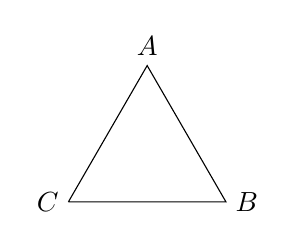
\begin{tikzpicture}
    \node[above](a) at (1,1.73){$A$};
    \node[right](b) at (2,0){$B$};
    \node[left](c) at (0,0){$C$};
    \draw(0,0)--(2,0)--(1,1.73)--(0,0);
    % \draw[dashed](0,0)--($(1,1.73)!(0,0)!(2,0)$);
    % \draw[dashed](2,0)--($(1,1.73)!(2,0)!(0,0)$);
    % \draw[dashed](1,1.73)--($(2,0)!(1,1.73)!(0,0)$);
\end{tikzpicture}
\end{center}
この三角形の持つ対称性,つまりこの幾何学的対象を「そのままに保つ」ような変換とはなんだろうか.
例えばいまあなたが目を閉じている間に,私が三角形を$120\times n$度(ただし$n$は整数)右に回転させても,目を開けたあなたは以前との違いに何も気が付かないだろう.
その意味で,$120\times n$度回転は正三角形をそのままに保つ変換=対称性である.
それ以外にも,それぞれの頂点から対辺の中間地点へとおろした軸に沿って線対称をとっても,図形は変わらない.
よってこうした鏡映反転も対称性である.
今,120度,240度の時計回り回転をそれぞれ$c_1, c_2$と表し,点$A, B, C$を通る軸に沿った鏡映反転をそれぞれ$\sigma_A, \sigma_B, \sigma_C$と表す.
これに「何もしない」変換(これはもちろん三角形をそのままに保つ)$i$を加えると,$\{i, c_1, c_2, \sigma_A, \sigma_B, \sigma_C\}$は群をなす.
この群の演算は下の積表によって表すことができる.
\[
\begin{array}{c|cccccc}
       & i & c_1 & c_2 & \sigma_A & \sigma_B & \sigma_C \\ \hline
       i & i & c_1 & c_2 & \sigma_A & \sigma_B & \sigma_C \\ 
       c_1 & c_1 & c_2 & i &  \sigma_C & \sigma_A & \sigma_B  \\ 
       c_2 & c_2 & i & c_1 &  \sigma_B & \sigma_C & \sigma_A \\ 
       \sigma_A & \sigma_A & \sigma_B & \sigma_C &  &  &  \\ 
       \sigma_B & \sigma_B & \sigma_C & \sigma_A & & &  \\ 
       \sigma_C & \sigma_C & \sigma_A & \sigma_B & &  &  \\ 
     
\end{array}
\]
例えば3列目($c_1$の列)は,120度右回転させた後で各行の変換を行うとどうなるか,ということを示している.
「何もしない」$i$の場合は当然$c_1$のままである.
$c_1$を再び適用すれば,240度右回転$c_2$になる.
一方240度右回転は120度左回転と同じなので,$c_2 \circ c_1 = i$,つまり$c_2$は$c_1$の逆元である.
また120度右回転の後に$A$軸で鏡映反転$\sigma_A$させることは,$C$軸での鏡映反転$\sigma_C$と同じことになる(実際に図などを用いて確認してみよう).
このようにして,他の組み合わせについても変換を合成した結果を調べることができる.(練習問題:右下の9つの空欄を埋めてみよう.)

さて,我々はモノイドのところでも積表を見た.
モノイドと群の積表の一番顕著な違いは,群の積表の各行・列には,必ず一回だけ単位元$i$が現れる,ということである.
単位元が現れるということは,そのペアが互いに逆元になっているということである.
よってこのことは,群の各元は必ず一つの逆元を持つ,という事実に対応している.
さらに注意してみれば,単位元に限らず,積表の各行・列はすべての元を,それぞれ一つだけ含んでいる,ということに気がつく.
これはこの群でたまたまそうなっているのではなく,すべての群に共通する性質である.

以上で我々が確認したのは次のことである.
(1) 対象に施してもその対象を変えないような変換を対称性ないし対称変換という.
(2) 対称変換を重ねて施したものも対称変換になる.
(3) 「何もしない」という変換も当然対称変換である.
(4) ある対称変換に対して,それを「キャンセル」するような逆変換が存在する.
これが,「対称変換は群の構造を持つ」ということの意味である.

さて,上の例は正三角形を保つような対称変換群であった.
図形が変われば,その対称性も当然異なる.
例えば$A$を頂点とする二等辺三角形では,$\{ \sigma_A, i\}$のみが対称変換である.
一方,円の場合はあらゆる角度の回転,および中心点を通るあらゆる軸での鏡映が対称変換になる.
この意味において,二等辺三角形よりも三角形が,そして三角形より円のほうがより対称的であると言える.
つまり対象の対称性は,その変換群によって定められている.

\begin{exercise}
    正方形および長方形の対称変換をそれぞれ確定せよ.
\end{exercise}

\begin{exercise}
    5章で見た準同型は,群についても同様にいえる.
    群$(G, \circ, i)$から群$(G', \circ', i')$への準同型写像とは,写像$f:G \to G'$であって,すべての$x, y \in G$について$f(x\circ y) = f(x) \circ' f(y)$が成立するものである.
    例えば上の正三角形と二等辺三角形の対象変換の間に,以下のような写像を構築すると,これは両群の間の準同型写像になっている:
    \[
    f(c_1)=f(c_2)=i, \ \ \ f(\sigma_1) = f(\sigma_2) = f(\sigma_3) = \sigma_A.    
    \]
    \begin{enumerate}
        \item これが準同型写像の定義を満たすことを確認せよ.
p        \item 上の練習問題で求めた正方形から長方形の対象変換群への準同型写像を構築せよ.
    \end{enumerate}
\end{exercise}



\section{対称性の哲学的含意}

対称性の問題は,陰に陽に,多くの哲学的議論で現れてくる.
またそれだけでなく,対称性は現代の数学・物理学においても非常に重要な概念である.
対称性の重要性が最初に明確に意識されたのは,19世紀後半に数学者のフェリックス・クラインが,弱冠23歳(!)でエルランゲン大学の教授に就任した際に提唱した,エルランゲン・プログラムである.
当時は,19世紀初頭の非ユークリッド幾何学の発見に導かれ,射影幾何学など様々な幾何学が林立していた.
クラインのプログラムは,こうした様々な幾何学を,対称性の観点から分類・統合する,というものである.
そのアイデアをざっくり説明すると,次のようなものである.
\begin{figure}[h]
\begin{center}
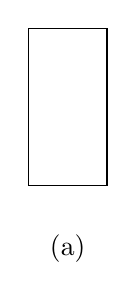
\begin{tikzpicture}
    \draw(0,0)--(1,0)--(1,2)--(0,2)--(0,0);
    \node[below](a) at (0.5,-.5){(a)};
\end{tikzpicture} 
\hspace{2em}
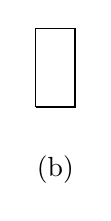
\begin{tikzpicture}
    \draw(0,0)--(0.5,0)--(0.5,1)--(0,1)--(0,0);
    \node[below](b) at (0.25,-.5){(b)};
\end{tikzpicture}
\hspace{2em}
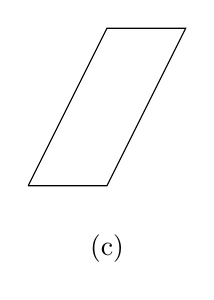
\begin{tikzpicture}
    \draw(0,0)--(1,0)--(2,2)--(1,2)--(0,0);
    \node[below](c) at (1,-.5){(c)};
\end{tikzpicture}
\hspace{2em}
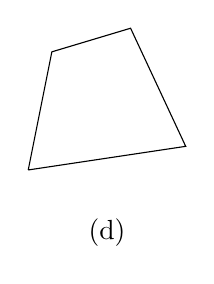
\begin{tikzpicture}
    \draw(0,0)--(2,0.3)--(1.3,1.8)--(0.3,1.5)--(0,0);
    \node[below](d) at (1,-.5){(d)};
\end{tikzpicture}
\hspace{2em}
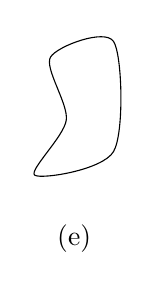
\begin{tikzpicture}
%    \draw plot[smooth cycle] coordinates{(0,0) (1,0) (2,1) (1,2)}
    \draw plot[smooth cycle] coordinates{(0,0) (1,0.3) (1,1.7)(.2,1.5)(.4,.7)};
    \node[below](e) at (.5,-.5){(e)};
\end{tikzpicture}
\end{center}
\caption{幾何学図形(長方形)に対する様々な変換.}
\label{erlangen}
\end{figure}

図\ref{erlangen}の左(a)に書かれた長方形は,様々な幾何学的性質を持っている.
まずそれは線で囲まれており,その線は4本の直線であり,対辺の長さは等しく,隣接した辺同士は直角で交わり,さらには各辺は具体的な長さ(印刷された用紙によって異なるだろうが,例えば長辺3cm)を持っている.
しかしこれらの性質全てが同じステータスを持っているわけではなく,いくつかはより「根源的」であるように思える.
この性質間の質的違いは,対称性の観点から理解できる.
例えば辺の長さは,相似変換によって変わってしまうが,それ以外の性質は不変に保たれる(b).
角度はアフィン変換(affine transformation)と呼ばれる変換により変わるが,対辺の長さが等しいという特徴は保たれる(c).
しかしその特徴も,ある光源から出た光でこの図形を他の面に射影する射影変換(projection transformation)では変わってしまう(d)(プロジェクタから斜めに投影するとスライドの画像がずれてしまうことを思い起こすとわかりやすい).
また最後に,位相のところで見た連続変換を施せば,不変にとどまる性質は「線で囲まれている」ということだけである(e).
これらの変換はそれぞれ,別個の(しがし互いにネストした)群を形成する.
そして上で述べた各性質は,異なる変換群に対する対称性を例示していると考えて良い.
クラインはこうした洞察から,幾何学とは,何らかの変換群に対して不変(invariant)にとどまる性質,すなわち対称性を探求する学問である,と特徴づけた(例えば射影幾何学は,射影変換に対して不変な性質を探求する).

逆に見れば,「幾何学的性質」というものは,変換群に対する対称性として定義することができる.
そして何が正真正銘の幾何学的性質とみなされるかは,扱う幾何学/変換群によって変わってくる.
例えば「角度」という概念は,ユークリッド幾何学では意味があるがアフィン幾何学では意味がない.
したがって,「正三角形」はユークリッド世界では客観的に存在するが,アフィン世界ではそうではない.
このように,性質やモノの実在性を対称性として特徴づけるアプローチは,数学に限らず,物理学でも重要な役割を担ってきた.
例えば古典物理学における物体(古典力学において「存在」するもの)は,ガリレオ変換とよばれる変換群に対して不変性を保つ.
一方,相対論において正真正銘のモノないし性質と認められるものは,それとは別の,ローレンツ変換に対して不変でなければならない.
ローレンツ変換は時間軸と空間軸を「混ぜる」変換なので,例えばものの「長さ」は相対論においては客観的な性質ではない(光速に近い速度で移動すると,同じものが違った長さに見える).

\begin{example}[有意味性と対称性]
京都の平均気温は4月は摂氏14度,8月は28度である.
しかしこれをこれをもって,「京都の8月は4月の2倍暑い」ということは意味をなさない.
というのも気温を華氏で表現すれば,それぞれ57度と82度になり,「2倍」という関係は成立しないからだ.
一般に,温度はアフィン変換$y = \alpha x + \beta$可能\footnote{例えば$y$を華氏,$x$を摂氏とすると,$y = 1.8x+32$.}なので,こうした変換において不変に保たれる性質のみが温度についての客観的性質として認められる.
アフィン変換は群をなすので\footnote{アフィン変換$y=\alpha x + \beta$を$(\alpha, \beta)$で表すと,単位元は$(1,0)$. $(\alpha, \beta), (\alpha',\beta')$という2つの変換に対し,合成は$(\alpha' \alpha, \alpha' \beta + \beta')$. 変換$(\alpha, \beta)$の逆元は$(1/\alpha, -\beta)$. 結合律については明らか.},これは対称性である.
ここから,ある対象(温度)についてどんな言明が有意味であるかは,その対象の対称性,すなわちそれが許容する変換群を定めればよい,という方針が従う.
これは測定理論(theory of measurement)の中心的な考え方である\citep[e.g,][]{Narens2007-ty}.
\end{example}


\begin{example}[対称性議論:逆転クオリア] 
逆に,対称変換は対象の本質を変えないのであるから,そうした変換によって変わるような性質は,実在的ないしは客観的な性質ではない,という議論戦略も存在する.そうした議論は一般に\emph{対称性議論}(symmetry argument)と総称される.
有名な対称性議論として\emph{逆転クオリア}(inverted qualia)がある.
通常の人間が「赤」と感じる波長の光を見ると,「緑」に見えるような人を考えよう.
そうした人は,我々が木の葉を見るときに感じる質感を熟れたリンゴを見るときに感じており,また逆もしかりであるが,しかし行動においては全く差異を見いだせないだろう(むしろクオリアが逆転しているのは\emph{あなた}かもしれない).
これは,「今,赤(緑)の質を感じている」という性質を互いに入れ替えるような変換(これは群である)は,人間の状態一般を不変に保つ対称性変換であるということである.
よってそうした変換において変化する性質は,実在的な性質ではない,したがってクオリアについての事実は存在しない.
これはクオリアについての対称性議論である.
\end{example}

\begin{example}[対称性議論:グルーパラドクス] 
今まで観測されたエメラルドはすべて緑greenであったとしよう.
ここから,「全てのエメラルドは緑である」と考えるのは妥当な帰納推論であるように思える.
しかしいま,「2025年以前に観測され緑であるものと,2025年以降に観測され青であるもの」を指すグルーgrueという述語を導入する.
すると今までに観測されたエメラルドはすべてグルーなので,「全てのエメラルドはグルーである」という仮説も同様に支持されそうに思えるが,これは明らかにおかしい.
一つの解決策は,「2025年」という特定の時間を含む述語はおかしい,と考えることかもしれない.
しかしいま,「2025年以前に観測され青であるものと,2025年以降に観測され緑であるもの」を指すブリーンbleenという述語を導入しよう.
すると述語「緑」は,「2025年以前に観測されグルーであるものと,2025年以降に観測されブリーンであるもの」というように定義し返される.つまりグルー/ブリーンを使う人からすれば,「緑」のほうこそ特定の時間を含んでしまっている!
これは\cite{Goodman1955-nr}によって提唱された,\emph{グルーパラドクス}と呼ばれる帰納推論の未解決問題である.
これは緑/青という述語と,グルー/ブリーンという述語は互いに変換可能であり,よって緑仮説とグリーン仮説では優劣をつけることができないはずだという,対称性議論として理解できる.
\end{example}

\begin{example}[還元主義]
我々は上で,考える対称性の違いにより幾何学的性質の「根源性」の度合いのようなものが考えられることを見た.
そして現代物理学において,実在的性質は対称性,つまり変換群に対する不変性として定義されることを見た.
同じようなことは,他の科学にもいえるだろうか.
例えば,何らかの変換群に対する不変性として化学的性質,生物学的性質,などを定義していくことは可能だろうか.

またさらに,そのように定義されたとき,それぞれの変換群は幾何学のときのような階層構造を持っているだろうか.
例えば,化学的・生物学的性質はローレンツ変換に対しては不変だと期待できるかもしれない(なぜならそれは物理的性質を不変に保つのだから).
同じように,生物学的性質は化学的変換に対して不変だろうか.
存在論的還元主義は,この問いに肯定的に答える:すなわちそれによれば,各科学分野における客観的性質は,その分野を特徴付ける変換群によって定義され,なおかつその変換群は階層的な構造を持っている.
\end{example}

\begin{exercise}
上で述べた変換群の階層構造を,群準同型の言葉で表わせ.
また群準同型が半順序を成すという練習問題5.3の結論は,還元主義的科学観に対しどのような含意を持つだろうか.
\end{exercise}

\begin{exercise}
還元主義に従い,ミクロ理論$T$の性質を特徴づける変換群$f$からマクロ理論$T'$の変換群$g$への準同型写像があると仮定しよう.
このとき,$T$と$T'$の性質の間にはどのような関係が成り立っているだろうか.
具体的には,準同型写像の存在は$T'$の性質が$T$の性質に付随(supervene)することを含意するだろうか.
また逆に,付随性が満たされるとき,$f$から$g$への準同型写像が存在するだろうか.
\end{exercise}


\bibliographystyle{apalike}
\bibliography{m4p}

\end{document}